\section{Modell}
\label{sec:modell}

In this section, the research variables and hypotheses are presented.


Table 2
Definitions of dimensions.

% Tabellenformat 2
\begin{table}[ht] 
\footnotesize
\caption{Definition der Dimensionen}
\label{tab:Dimensionen} 
\begin{tabular}{@{}lp{9cm}l@{}} \toprule

\textbf{Konstrukt} & \textbf{Definiton} & \textbf{Quelle} \\ \midrule

Servicequalität & The quality of the support that users receive from e-learning system & \parbox[t]{4cm}{\cite{petter2008measuring}}\\ 
Systemqualität & The desirable characteristics and features of e-learning system and components & \parbox[t]{4cm}{\cite{petter2008measuring}}\\ Nutzerzufriedenheit & The extent to which users believe that their needs, goals, and desires have been fully met through using the e-learning system & \parbox[t]{4cm}{\cite{sanchez2009moderating}}\\ 
Persönlicher Nutzen & \parbox[t]{9cm}{tbd}  & \parbox[t]{4cm}{tbd} \\ \addlinespace 
  \bottomrule

\end{tabular}	
\end{table}


\begin{figure}[h]
\centering
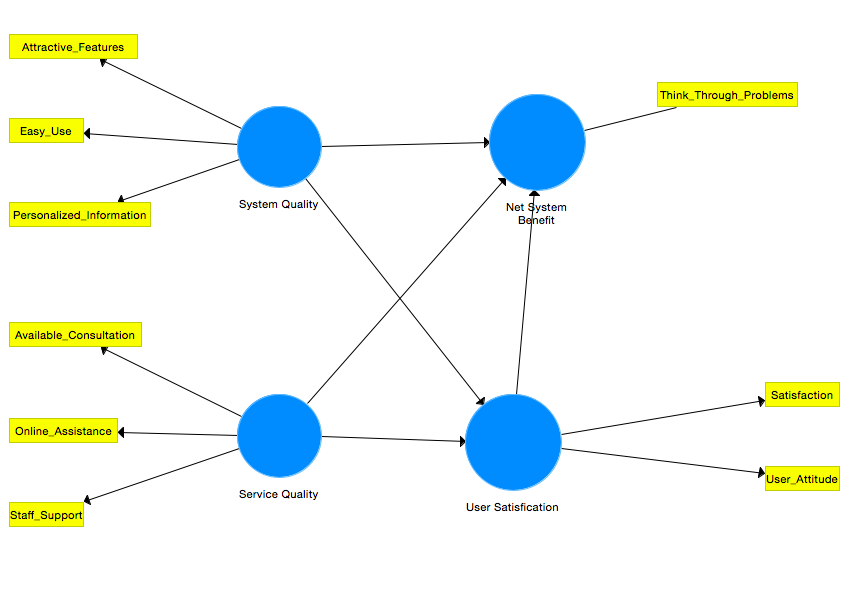
\includegraphics[width=1\textwidth]{Grafiken/Research_Model.png}
\caption{Research Model}
\label{Research Model}
\end{figure}